\chapter{Guia de Referencia}

El presente capitulo no pretende ser un completo manual de usuario de la aplicación, el sistema en si es bastante intuitivo en cuanto a su funcionamiento por lo que en este capítulo se resumirá un poco algunas de las diferentes sesiones y funcionalidades de la aplicación.

\section{Organización de la Aplicación}

La aplicación se organiza de la siguiente manera, con las diferentes aéreas bien definidas:

\begin{itemize}
    \item 1 Menú Principal
    \item 2 Menú Secundario
    \item 3 Cuerpo de la Aplicación
    \item 4 Información de Usuario
\end{itemize}

\begin{figure}[H]
    \centering
    \includegraphics[scale=0.5]{resourse/organizacion.png}
    \caption{Organización Espacial del contenido de la aplicación}
    \label{fig:61}
\end{figure}


\subsection{Menú Principal}

El contenido del menú principal depende del tipo de usuario que haya iniciado sesión en base a ello tendrá o no habilitadas diferentes funcionalidades de la aplicación, los único menús comunes son \textbf{Mensajes} y \textbf{Opciones}.


\subsection{Menú Secundario}

El menú secundario dependiendo de la vista donde se este, puede o no existir, y su contenido dependerá del las acciones que pueden ser realizadas en ella.


\subsection{Cuerpo de la Aplicación}

Aquí se localizara el contenido principal de la vista, ya sea un formulario para registrar alguna información, una lista para mostrar información etc.


\subsection{Información de Usuario}

Muestra información acerca de la sesión de usuario actual que se está ejecutando, tal información es el nombre del usuario \footnote{nombre real, no el usename} y el tipo de usuario que puede ser (Paciente, Medico, Administrativo, Not Login en caso de no haber
iniciado sesión)


\section{Panel de Usuario No Registrado}

Corresponde al panel que vera el usuario la primera vez que ingrese a la aplicación las funciones que se pueden hacer son restringidas y se limitan a:

\begin{itemize}
    \item \textbf{Inicio}: Ir a la pantalla de Inicio
    \item \textbf{Listado de Médicos}: Mostrar información básica acerca de los especialistas con los que cuenta la institución.
    \item \textbf{Registrarse}: Permite al usuario mediante una serie de pasos registrarse como paciente.
    \item \textbf{Iniciar Sesión}: Iniciar una sesión con un usuario registrado.
\end{itemize}

En cuanto la vista \textbf{Inicio} es solo la pantalla principal de presentación de la aplicación con un logo de fondo.

La vista \textbf{Listado de Médicos} puede consultarla en la sesión del panel del Paciente, ya que la única diferencia considerable es que se agregan un par de opciones que permiten al Paciente realizar algunas acciones a diferencia del usuario no registrado que solo puede visualizar parte de la información.


\subsection{Registrarse}

Esta vista ofrece a los usuarios no registrados, un formulario donde deberán cargar una serie de datos para registrarse como pacientes.

\begin{figure}[H]
    \centering
    \includegraphics[scale=0.5]{resourse/registrar-paciente.png}
    \caption{Formulario Registro Paciente}
    \label{fig:62}
\end{figure}

Completado el registro y luego de enviado el formulario, si todos los datos son correctos nos mostrara un mensaje de que el registro fue exitoso:

\begin{figure}[H]
    \centering
    \includegraphics[scale=0.5]{resourse/registro-exito.png}
    \caption{Formulario Registro Paciente}
    \label{fig:63}
\end{figure}

Paso siguiente deberemos revisar nuestra casilla de correo donde nos aparecerá el mensaje con la dirección del formulario para activación de usuario. \footnote{Si se intenta iniciar sesión sin haber activado el usuario nos devolverá un mensaje de error.}.

\begin{figure}[H]
    \centering
    \includegraphics[scale=0.5]{resourse/correo-bandeja.png}
    \caption{Bandeja de Correo con el mensaje}
    \label{fig:64}
\end{figure}

\begin{figure}[H]
    \centering
    \includegraphics[scale=0.5]{resourse/correo-mensaje.png}
    \caption{Cuerpo del mensaje con la información de activación de usuario}
    \label{fig:65}
\end{figure}

\begin{figure}[H]
    \centering
    \includegraphics[scale=0.5]{resourse/usuario-activar.png}
    \caption{Formulario de Activación de usuario}
    \label{fig:66}
\end{figure}

Luego de estos pasos el usuario estará registrado y activado, solo faltaría iniciar sesión para poder empezar a operar como paciente.

\subsection{Iniciar Sesión}

La vista de inicio de sesión no es nada de otro mundo, solo es un simple formulario donde debes introducir el usuario y contraseña validos para poder iniciar sesión.


\section{Panel de Usuario Paciente}

Corresponde al panel de funciones al que tendrán acceso los usuarios, pacientes sigue siendo limitado pero ya se pueden hacer algunas cosas como solicitar turnos y realizar consultas médicas rápidas a un especialista, se organiza en:

\begin{itemize}
    \item \textbf{Inicio}: Ir a la pantalla de Inicio
    \item \textbf{Listado de Médicos}: Mostrar información  acerca de los especialistas.
    \item \textbf{Mensajes}: Casilla de Mensajes Internos.
    \item \textbf{Mis Turnos}: Información acerca del estado de los turnos del usuario.
    \item \textbf{Opciones}: Panel de Opciones
\end{itemize}


\subsection{Listado de Médicos}

Vista que permite seleccionar entre el listado de especialistas que componen el cuerpo médico de la institución consultar información, realizar una consulta rápidas y solicitar turno.

\begin{figure}[H]
    \centering
    \includegraphics[scale=0.5]{resourse/listado-medico.png}
    \caption{Listado de Médicos}
    \label{fig:67}
\end{figure}

\begin{figure}[H]
    \centering
    \includegraphics[scale=0.5]{resourse/consulta-online.png}
    \caption{Formulario de Consulta Online}
    \label{fig:68}
\end{figure}

\begin{figure}[H]
    \centering
    \includegraphics[scale=0.5]{resourse/medico-mostrar.png}
    \caption{Mostrar Datos del Medico}
    \label{fig:69}
\end{figure}

La vista de Asignación de turno son similares, entre si no varían mucho por lo que se explicara en la parte del panel de Medico.


\subsection{Mensajes}

Como ya se menciono esto es una sesión común a todas los usuarios, se trata de un conjunto de vista donde funciona el sistema de mensajería interna entre los usuarios de la aplicación, su función está reducida en cuanto al usuario paciente ya que este solo puede visualizar y responder los mensajes que se le envían, para enviar un mensaje a un profesional se realiza mediante la opción de realizar consulta online, por lo que solo puede enviar mensaje a los especialistas, las opciones disponible son:

\begin{itemize}
    \item \textbf{Redactar}: Escribir un Nuevo Mensaje
    \item \textbf{Recibidos}: Bandeja de Entrada
    \item \textbf{Enviado}: Bandeja de Salida
\end{itemize}

Algunas de las cuales pueden ser apreciadas en las siguientes capturas:

\begin{figure}[H]
    \centering
    \includegraphics[scale=0.5]{resourse/mensaje-redactar.png}
    \caption{Redactar un Mensaje}
    \label{fig:610}
\end{figure}

\begin{figure}[H]
    \centering
    \includegraphics[scale=0.5]{resourse/mensaje-recibidos.png}
    \caption{Bandeja de Entrada}
    \label{fig:611}
\end{figure}

\begin{figure}[H]
    \centering
    \includegraphics[scale=0.5]{resourse/mensaje-mostrar.png}
    \caption{Mostrar Mensaje}
    \label{fig:612}
\end{figure}

\subsection{Opciones}
Otro menú común a todos los usuarios permite la administración de los datos e información del mismo, dentro de las funciones que permite este menú se encuentra:

\begin{itemize}
    \item \textbf{Mis Datos}: Mostrar/Modificar Datos personales
    \item \textbf{Cambiar Contrase\~na}: Formulario para cambio de Contrase\~na
    \item \textbf{Cerrar Sesión}: Cerrar Sesión, despedirse del sistema.
\end{itemize}


\section{Panel de Usuario Administrativo}

Corresponde al panel de funciones al que tendrán acceso los usuarios administrativos .

\begin{itemize}
    \item \textbf{Inicio}: Ir a la pantalla de Inicio
    \item \textbf{Pacientes}: Administrar Usuarios Pacientes
    \item \textbf{Médicos}: Administrar usuarios Médicos
    \item \textbf{Administrativos}: Administrar usuarios Administrativos
    \item \textbf{Especialidades}: Administrar especialidades medicas
    \item \textbf{Mensajes}: Casilla de mensajes Internos.
    \item \textbf{Opciones}: Panel de opciones
\end{itemize}


\subsection{Pacientes, Médicos, Administrativos}

Los tres conjuntos de vistas comparten muchas características similares por lo que se explican en conjunto y solo se mencionaran algunas de sus diferencias, cada sub menú se enlista de acuerdo a los tipos de usuarios que se desea administrar, permitiendo según el sub menú la posibilidad de crear un tipo de usuario especifico \footnote{Los Usuarios registrados por el Administrador o el médico no requieren activación como los usuarios creados por usuarios no registrados.} Buscar un usuario, modificar sus datos.


\begin{figure}[H]
    \centering
    \includegraphics[scale=0.5]{resourse/datos-admin.png}
    \caption{Mostrar Administrativo}
    \label{fig:615}
\end{figure}

\begin{figure}[H]
    \centering
    \includegraphics[scale=0.5]{resourse/listado-paciente.png}
    \caption{Vista para búsqueda de usuario, en este caso usuarios Pacientes}
    \label{fig:616}
\end{figure}

En el caso de los usuarios médicos además puede consultar y modificar el estado de los turnos que les fueron solicitados, definirles especialidades correspondiente.

\begin{figure}[H]
    \centering
    \includegraphics[scale=0.5]{resourse/datos-medico-a.png}
    \caption{Mostrar Medico}
    \label{fig:614}
\end{figure}


\begin{figure}[H]
    \centering
    \includegraphics[scale=0.5]{resourse/turnos-sol-medico.png}
    \caption{Vista Listado Turnos Solicitados al Medico.}
    \label{fig:617}
\end{figure}


En los pacientes además puede asignar un turno a los mismo, cancelar un turno solicitado por el mismo, mostrar información e imprimir comprobante correspondiente.

\begin{figure}[H]
    \centering
    \includegraphics[scale=0.5]{resourse/datos-paciente-a.png}
    \caption{Mostrar Paciente}
    \label{fig:613}
\end{figure}



\section{Panel de Usuario Médicos}

Corresponde al panel de funciones al que tendrán acceso los usuarios médicos aunque comparte funcionalidades en común con los otros paneles, presenta vistas exclusivas para el uso por parte de los médicos.

\begin{itemize}
    \item \textbf{Inicio}: Ir a la pantalla de Inicio
    \item \textbf{Cronograma}: Vista con las actividades pendiente para el día.
    \item \textbf{Pacientes}: Administrar Usuarios Pacientes
    \item \textbf{Turnos}: Información acerca del estado de los turnos del médico.
    \item \textbf{Mensajes}: Casilla de Mensajes Internos.
    \item \textbf{Opciones}: Panel de Opciones
\end{itemize}

\subsection{Cronograma}

La funcionalidad de esta vista es permitir un acceso rápido a la funciones comunes, mostrar los mensajes sin leer, y los turnos solicitados para la fecha.

\begin{figure}[H]
    \centering
    \includegraphics[scale=0.5]{resourse/cronograma.png}
    \caption{Vista del Cronograma}
    \label{fig:614}
\end{figure}


\subsection{Pacientes}

La colección de vistas correspondientes a los pacientes son similares a las vistas que presenta el rol administrativo, como se menciono antes el médico también puede registrar nuevos pacientes, lo que diferencia a las vistas de medico correspondiente a esta sesión es que ahora muestra un menú más amplio de opciones en comparación a la del administrador, se habilita el submenú para administrar lo referente a la
Historia clínica del paciente.

\begin{figure}[H]
    \centering
    \includegraphics[scale=0.5]{resourse/datos-paciente-m.png}
    \caption{Mostrar Paciente}
    \label{fig:615}
\end{figure}

La Primera parte corresponde al registro de información relevante obtenida durante la consultas medicas y prescripciones medicas \footnote{Lo que comúnmente se conoce como receta médica.} además de generar el comprobante para el paciente.

\begin{figure}[H]
    \centering
    \includegraphics[scale=0.5]{resourse/consulta-medica.png}
    \caption{Consulta Médica}
    \label{fig:616}
\end{figure}

\begin{figure}[H]
    \centering
    \includegraphics[scale=0.3]{resourse/receta.png}
    \caption{Imprimir Receta o Prescripción Medica}
    \label{fig:617}
\end{figure}

En cuanto a los estudios clínicos que se registran en la historia clínica, por lo general al seleccionarlo puede que se visualice: 


La información del examen únicamente, con la opción de modificación si este es único, por ejemplo el caso de registro de antecedentes perinatales.

\begin{figure}[H]
    \centering
    \includegraphics[scale=0.5]{resourse/modificar-perinatales.png}
    \caption{Examen Único}
    \label{fig:618}
\end{figure}

O también muestre un listado con los exámenes realizados donde se deberá seleccionar el examen especifico que se desea consultar, o registrar un nuevo examen en caso de requerirlo, como por ejemplo es el caso del examen físico ya que al paciente pueden realizarle durante su vida varios exámenes de este tipo.

\begin{figure}[H]
    \centering
    \includegraphics[scale=0.5]{resourse/listado-cardio.png}
    \caption{Listado de Exámenes Aparato Cardiovascular}
    \label{fig:619}
\end{figure}

\begin{figure}[H]
    \centering
    \includegraphics[scale=0.5]{resourse/detalle-cardio.png}
    \caption{Vista Muestra Datos Examen Cardiovascular}
    \label{fig:620}
\end{figure}

\begin{figure}[H]
    \centering
    \includegraphics[scale=0.5]{resourse/nuevo-fisico.png}
    \caption{Nuevo Examen Físico}
    \label{fig:621}
\end{figure}


\subsection{Turnos}

\subsubsection{Registrar nuevo Turno}

El procedimiento relacionado al registro de un nuevo turno es similar en todos los casos solo tiene pequeñas variaciones dependiendo el rol del usuario, si se es paciente por ejemplo se seleccionara el médico al que se desea solicitar el turno, en caso de ser medico seleccionara el paciente, y si es administrativo seleccionara ambos (médico y paciente), luego el sistema le mostrara un calendario con las posibles fechas (fig:622) donde puede solicitar un turno dependiendo de los días de atención que el médico haya estipulado.

\begin{figure}[H]
    \centering
    \includegraphics[scale=0.5]{resourse/calendario.png}
    \caption{Vista para Selección de día de calendario para Asignar turno}
    \label{fig:622}
\end{figure}

Luego de seleccionada la fecha entre las disponible se muestra una vista con el resumen de la información del paciente, medico, la fecha \footnote{El horario recién se define cuando el turno es registrado.} donde se debe confirmar el registro del turno, este paso es obligatorio para evitar registrar accidentalmente un turno.

\begin{figure}[H]
    \centering
    \includegraphics[scale=0.5]{resourse/confirmacion-turno.png}
    \caption{Vista de Confirmación de los datos del Turno}
    \label{fig:623}
\end{figure}

Después de confirmado, se mostraran los datos completo del turno, así como la opción de imprimir un comprobante.


\begin{figure}[H]
    \centering
    \includegraphics[scale=0.5]{resourse/datos-turno.png}
    \caption{Vista muestra la informacion del Turno}
    \label{fig:624}
\end{figure}


\begin{figure}[H]
    \centering
    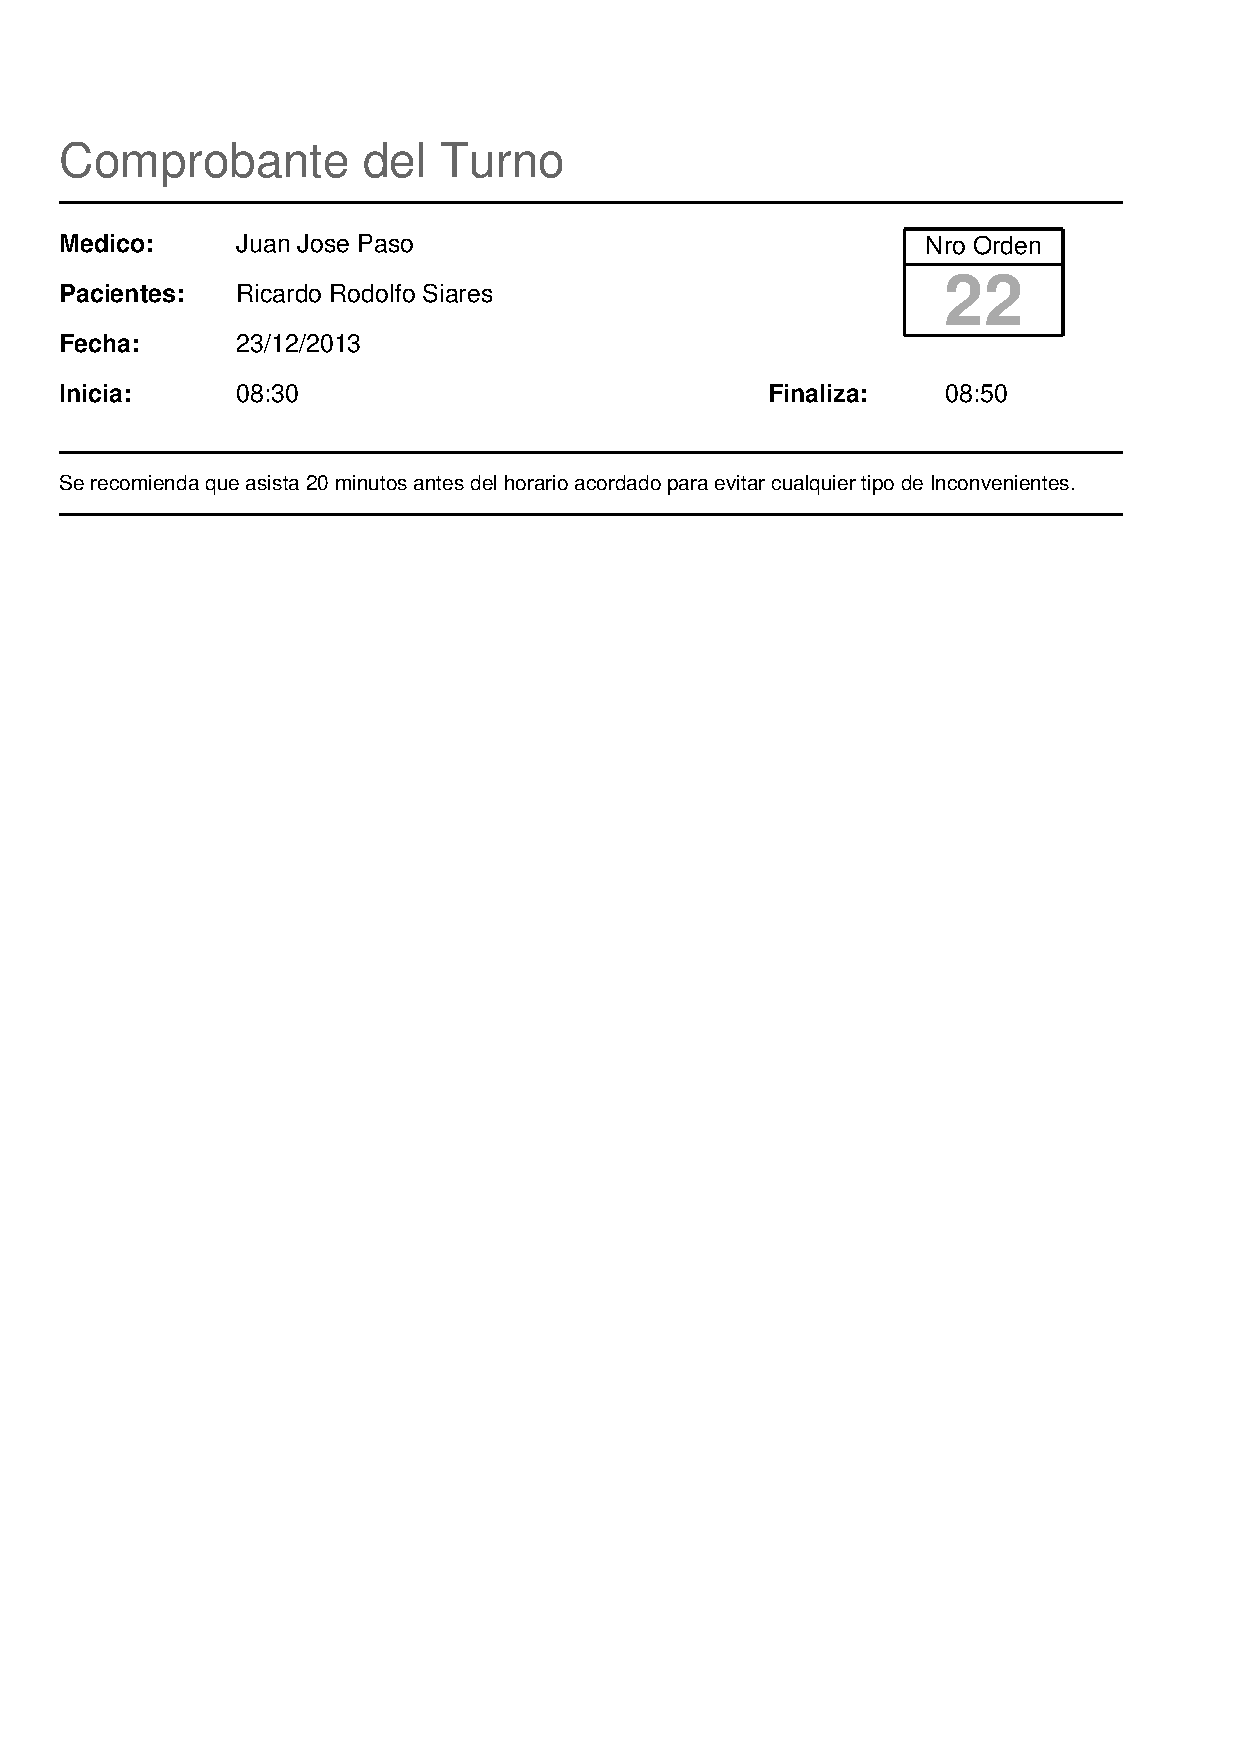
\includegraphics[scale=0.5]{resourse/comprobante-turno.png}
    \caption{Ejemplo de Comprobante de turno}
    \label{fig:625}
\end{figure}

Con esto último, se concluye esta pequeña guía de uso del sistema.













